\documentclass[t, notes, xcolor=table]{beamer}

\usepackage{wrapfig}
\usepackage{float}
% For tabs in verbatim
\usepackage{fancyvrb}

% Adjust position of the image
\usepackage[export]{adjustbox}

% set fonts
\usefonttheme{professionalfonts} % using non standard fonts for beamer
\usepackage{txfonts,mathptmx}

% set indend spacing for first and second level indentation
\setlength{\leftmargini}{0.5cm}
\setlength{\leftmarginii}{0.5cm}
\setlength{\leftmarginiii}{0.5cm}

% Set circles for bullets 
\setbeamertemplate{itemize items}[circle]

% colors
\usepackage{xcolor}

% multiple columns
\usepackage{multicol}

% todo lists
\usepackage{pifont}
\usepackage{amssymb}

% increase space between text and frame name
\addtobeamertemplate{frametitle}{}{\vspace{0.5em}}

%Information to be included in the title page:
\title{Making Procedural Statements}
\author{Nikola Petrovic}
\institute{University of Belgrade, School of Electrical Engineering}
\date{2022}



\begin{document}

\frame{\titlepage}

%%%%%%%%%%%%%%%%%%%%%%%%%%%%%%%%%%%%%%%%%%%%%%%%%%%%%%%%%%%%
\begin{frame}
\frametitle{Module Objective}

In this module we will describe design behaviour procedurally.
\textbf{Topics:}
\begin{itemize}
\item Procedural blocks review
\item Making procedural statements
\item Making conditional statements
\item Making case statements
\item Making loop statements
\end{itemize}

\end{frame}
\note{
Out objective is to appropriately and effectively procedurally describe design behaviour. To do that, we need to know generally about procedural blocks and procedural statements, and more specifically about branching procedural statements. The Verilog behavioural modeling constructs are very similar to the C programming language. They differ in subtle ways that can sometimes be irksome.
}

%%%%%%%%%%%%%%%%%%%%%%%%%%%%%%%%%%%%%%%%%%%%%%%%%%%%%%%%%%%%
\begin{frame}
\frametitle{Describing Module Behaviour}

\begin{itemize}
\item The \textcolor{purple}{initial} construct starts execution at the start of the simulation, and when complete, terminates the process.
\item The \textcolor{purple}{always} construct starts execution at the start of the simulation, and when complete, executes again.

\begin{figure}
    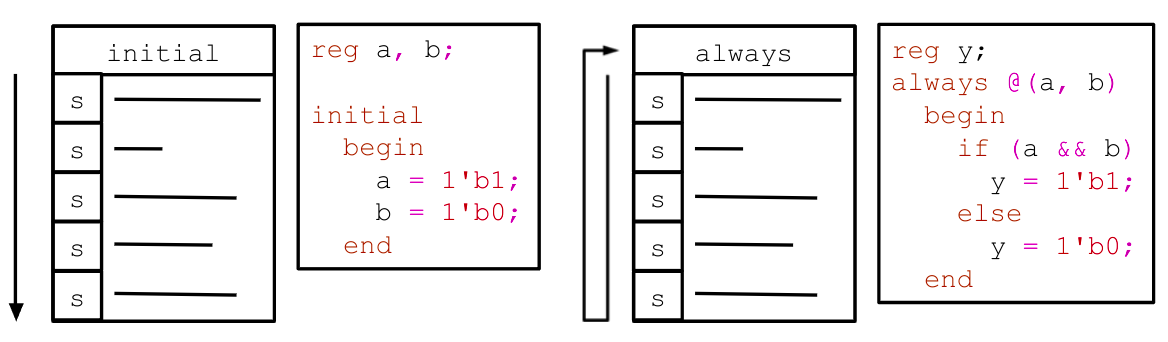
\includegraphics[width=0.95\textwidth]{img/06_mod_beh.png}
\end{figure}
\end{itemize}
\end{frame}
\note{
\scriptsize{
Event simulation relies upon processes. A process is an object that reacts to input events and generates output events. The continuous assignment that we have already seen is a process - the simulator reacts to its input transitions to calculate new output value and transitions the net to that new value.
\newline

Verilog has other kinds of processes - two most obvious to the user are the \textbf{initial} construct and the \textbf{always} construct, frequently referred to as the initial and the always block. The \textit{initial} and \textit{always} keywords are not statements themselves - they apply to their following statement and make it execute as a process. Their following statement is usually a statement block, e.g., statements between the \textit{begin} and \textit{end} keywords, but does not have to be.
\begin{itemize}
\item The simulator executes each \textit{initial} process at the start of the simulation, and upon completing its execution, terminates the process.
\item The simulator executes each \textit{always} process at the start of the simulation, and upon completing its execution, executes it again.
\end{itemize}

}
}

%%%%%%%%%%%%%%%%%%%%%%%%%%%%%%%%%%%%%%%%%%%%%%%%%%%%%%%%%%%%
\begin{frame}
\frametitle{Synchronizing Module Behaviours}
\scriptsize{
\begin{multicols}{2}
\begin{itemize}
\item Procedures "block" upon encountering an event control
\item Procedures "unblock" upon occurrence of any of the listed events.
\item An event control can reference:
\begin{itemize}
\scriptsize{
	\item A single event identifier
	\item An event expression
	\item The "$*$" wildcard operator
}
\end{itemize}

\end{itemize}
\vfill
\columnbreak
\begin{figure}
    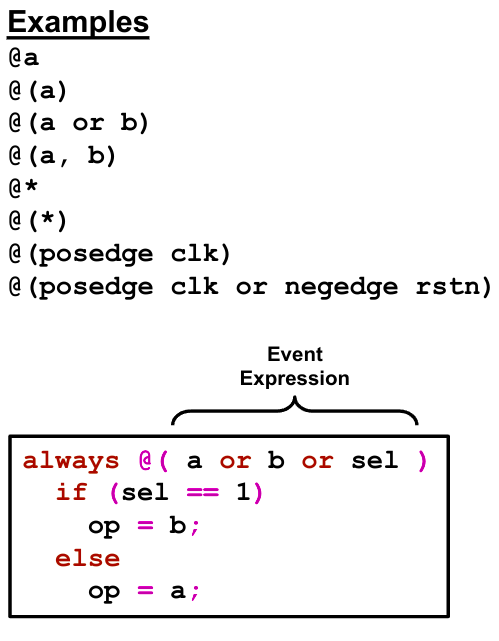
\includegraphics[width=0.45\textwidth]{img/06_sync.png}
\end{figure}
\end{multicols}
}
\end{frame}
\note{
\scriptsize{
If an \textbf{always} construct has no constructs to block it execution, then when the simulator started executing it at the start of simulation, execution would continue in a tight loop forever and the simulator would appear to hang.
\newline

Verilog provides procedural timing controls for "stepping" execution of procedural blocks. The most common of these is the event control. An event control starts with the \textbf{at (@)} character and then follows with either a wildcard character, a single event identifier, or a parenthesized event expression. The event expression can be a list of event expressions separated by the \textbf{or} keyword or by the comma (,) character. Both are shown in the example. The \textbf{or} keyword in an event expression is a separator between event expressions and is not an operator in the usual sense. We can further qualify an expression with the \textbf{posedge} or \textbf{negedge} keywords.
\newline

A timing control is not itself a statement, but precedes a statement, and in the case of an event control, blocks execution of that statement and subsequent sequential statements until on of those events occur.

}
}


%%%%%%%%%%%%%%%%%%%%%%%%%%%%%%%%%%%%%%%%%%%%%%%%%%%%%%%%%%%%
\begin{frame}
\frametitle{Interactions Between Behaviours}
\begin{figure}
    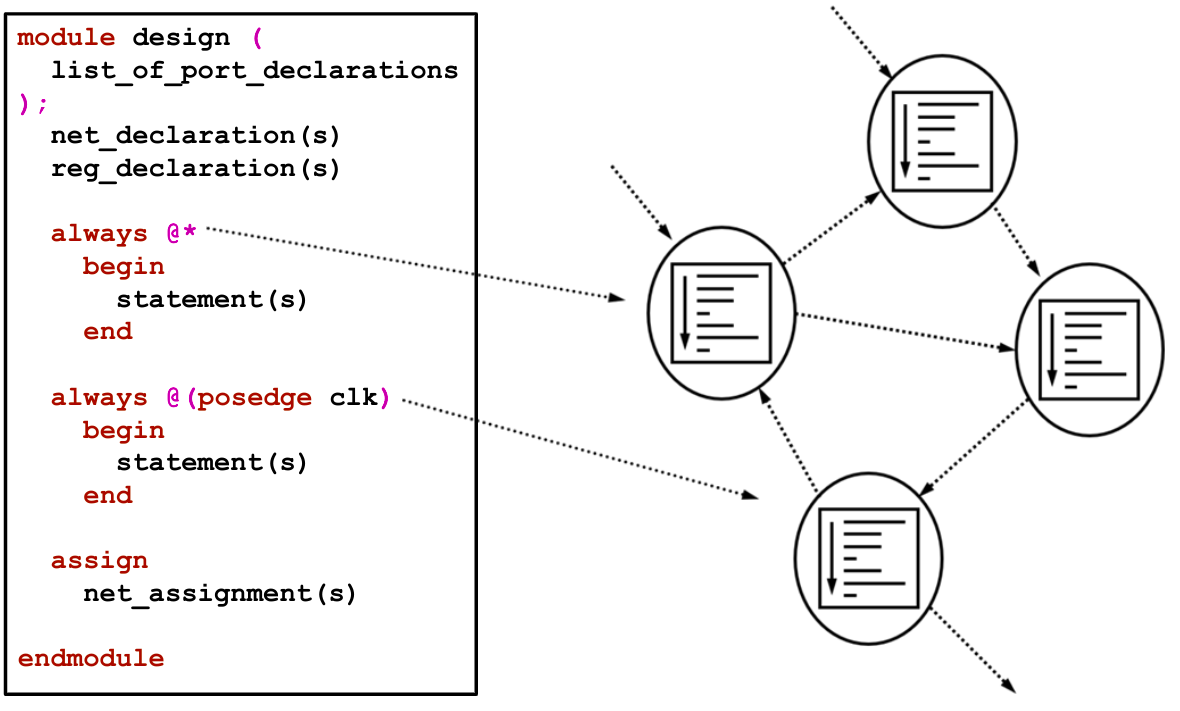
\includegraphics[width=0.95\textwidth]{img/06_interaction.png}
\end{figure}
\end{frame}
\note{
\scriptsize{
A non-trivial design usually contains several modules, and a module at the RT level typically contains procedural blocks:
\begin{itemize}
\item Each sequential procedural block executes its statement sequentially like a conventional programming language.
\item Multiple blocks execute concurrently, like hardware.
\item Multiple blocks communicate with each other using events, nets and variables.
\end{itemize}

The capability to have many procedural blocks communicating concurrently with each other is the basic model which Verilog uses to describe hardware.
}
}

%%%%%%%%%%%%%%%%%%%%%%%%%%%%%%%%%%%%%%%%%%%%%%%%%%%%%%%%%%%%
\begin{frame}
\frametitle{Making Procedural Assignments}

\end{frame}

%%%%%%%%%%%%%%%%%%%%%%%%%%%%%%%%%%%%%%%%%%%%%%%%%%%%%%%%%%%%
\begin{frame}
\frametitle{Module}

\end{frame}

%%%%%%%%%%%%%%%%%%%%%%%%%%%%%%%%%%%%%%%%%%%%%%%%%%%%%%%%%%%%
\begin{frame}
\frametitle{Module}

\end{frame}

%%%%%%%%%%%%%%%%%%%%%%%%%%%%%%%%%%%%%%%%%%%%%%%%%%%%%%%%%%%%
\begin{frame}
\frametitle{Module}

\end{frame}

%%%%%%%%%%%%%%%%%%%%%%%%%%%%%%%%%%%%%%%%%%%%%%%%%%%%%%%%%%%%
\begin{frame}
\frametitle{Module}

\end{frame}


\end{document}
